%!tex ts-program = xelatex
%!tex encoding = utf-8 unicode

\documentclass{htw}

\htwCourse{Special Computer Engineering}
\htwTopic{Bau eines VHDL-Automaten Generators}
\htwDate{\today}

\htwTitle{Hopperlang}
\htwSubtitle{- simple state machines -}

\htwAddAuthor{Pedro}{Scaff}
\htwAddAuthor{Lukas}{Jünemann}
\htwAddAuthor{Robert}{Günzler}
\htwAddAuthor{Fatih}{Duran}
\htwAddAuthor{Christoph}{Franke}

% 1. 
% Theorethischer Abriss, Compilerbau-Kernkomponenten, 
% Entweder am konktreten Werkzeug oder nicht
% 2. 
% Abriss Kernaufgabe: Automaten Transformationssprache
% 3. 
% Die von uns entwickelte Sprache, wieso der Aufbau, 
% in relation zum Aufbau eines Automaten und wie werden diese 
% Automaten-Komponenten dargestellt.
% 4. 
% Aufbau unseres Compilers, aus welchen Komponenten besteht dieser 
% (was geht rein, was kommt raus, Zusammenfassung)

\begin{document}
\maketitle
% \captionsetup{justification=raggedleft,singlelinecheck=false}


% start here
\section{Theoretische Grundlagen}

\subsection{Lexikalische Analyse}

\blockquote[André Platzer, Compiler Design\footnote{\url{https://www.cs.cmu.edu/~fp/courses/15411-f13/lectures/07-lex.pdf}}]{
Lexical analysis is the first phase of a compiler. Its job is to turn a raw byte or character input stream coming from the source file into a token stream by chopping
the input into pieces and skipping over irrelevant details.  
}

\begin{figure}[h]
    \centering
    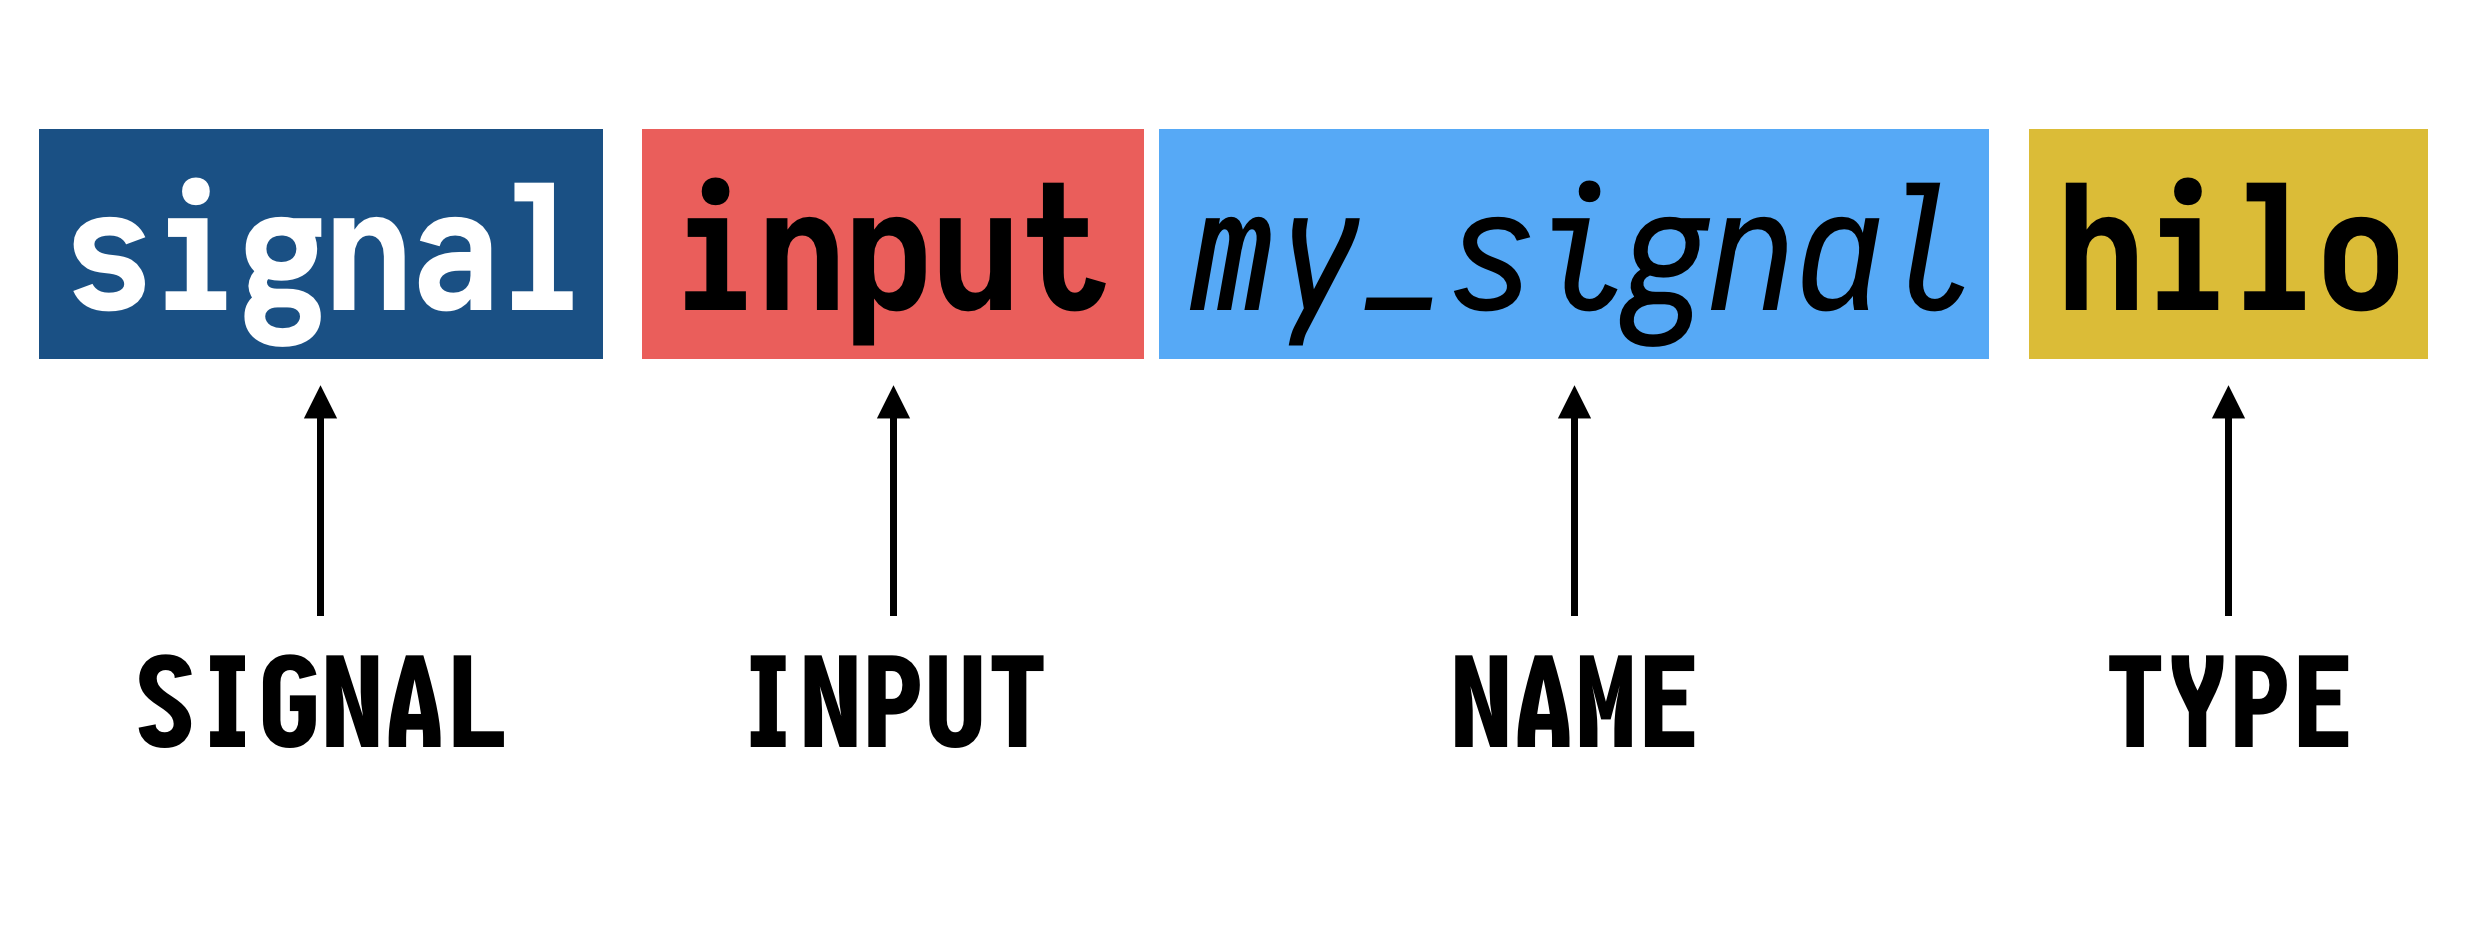
\includegraphics[height=5cm]{res/lexer.png}
    \caption{Beispiel: Hopperlang lexing}\label{fig:lex}
\end{figure}

\subsection{Syntaktische Analyse}

\blockquote[Wikipedia, Compiler\footnote{\url{https://en.wikipedia.org/wiki/Compiler}}]{
Syntax analysis involves parsing the token sequence to identify the syntactic structure of the program. This phase typically builds a parse tree, which replaces the linear sequence of tokens with a tree structure built according to the rules of a formal grammar which define the language's syntax.
}

\begin{figure}[h]
    \centering
    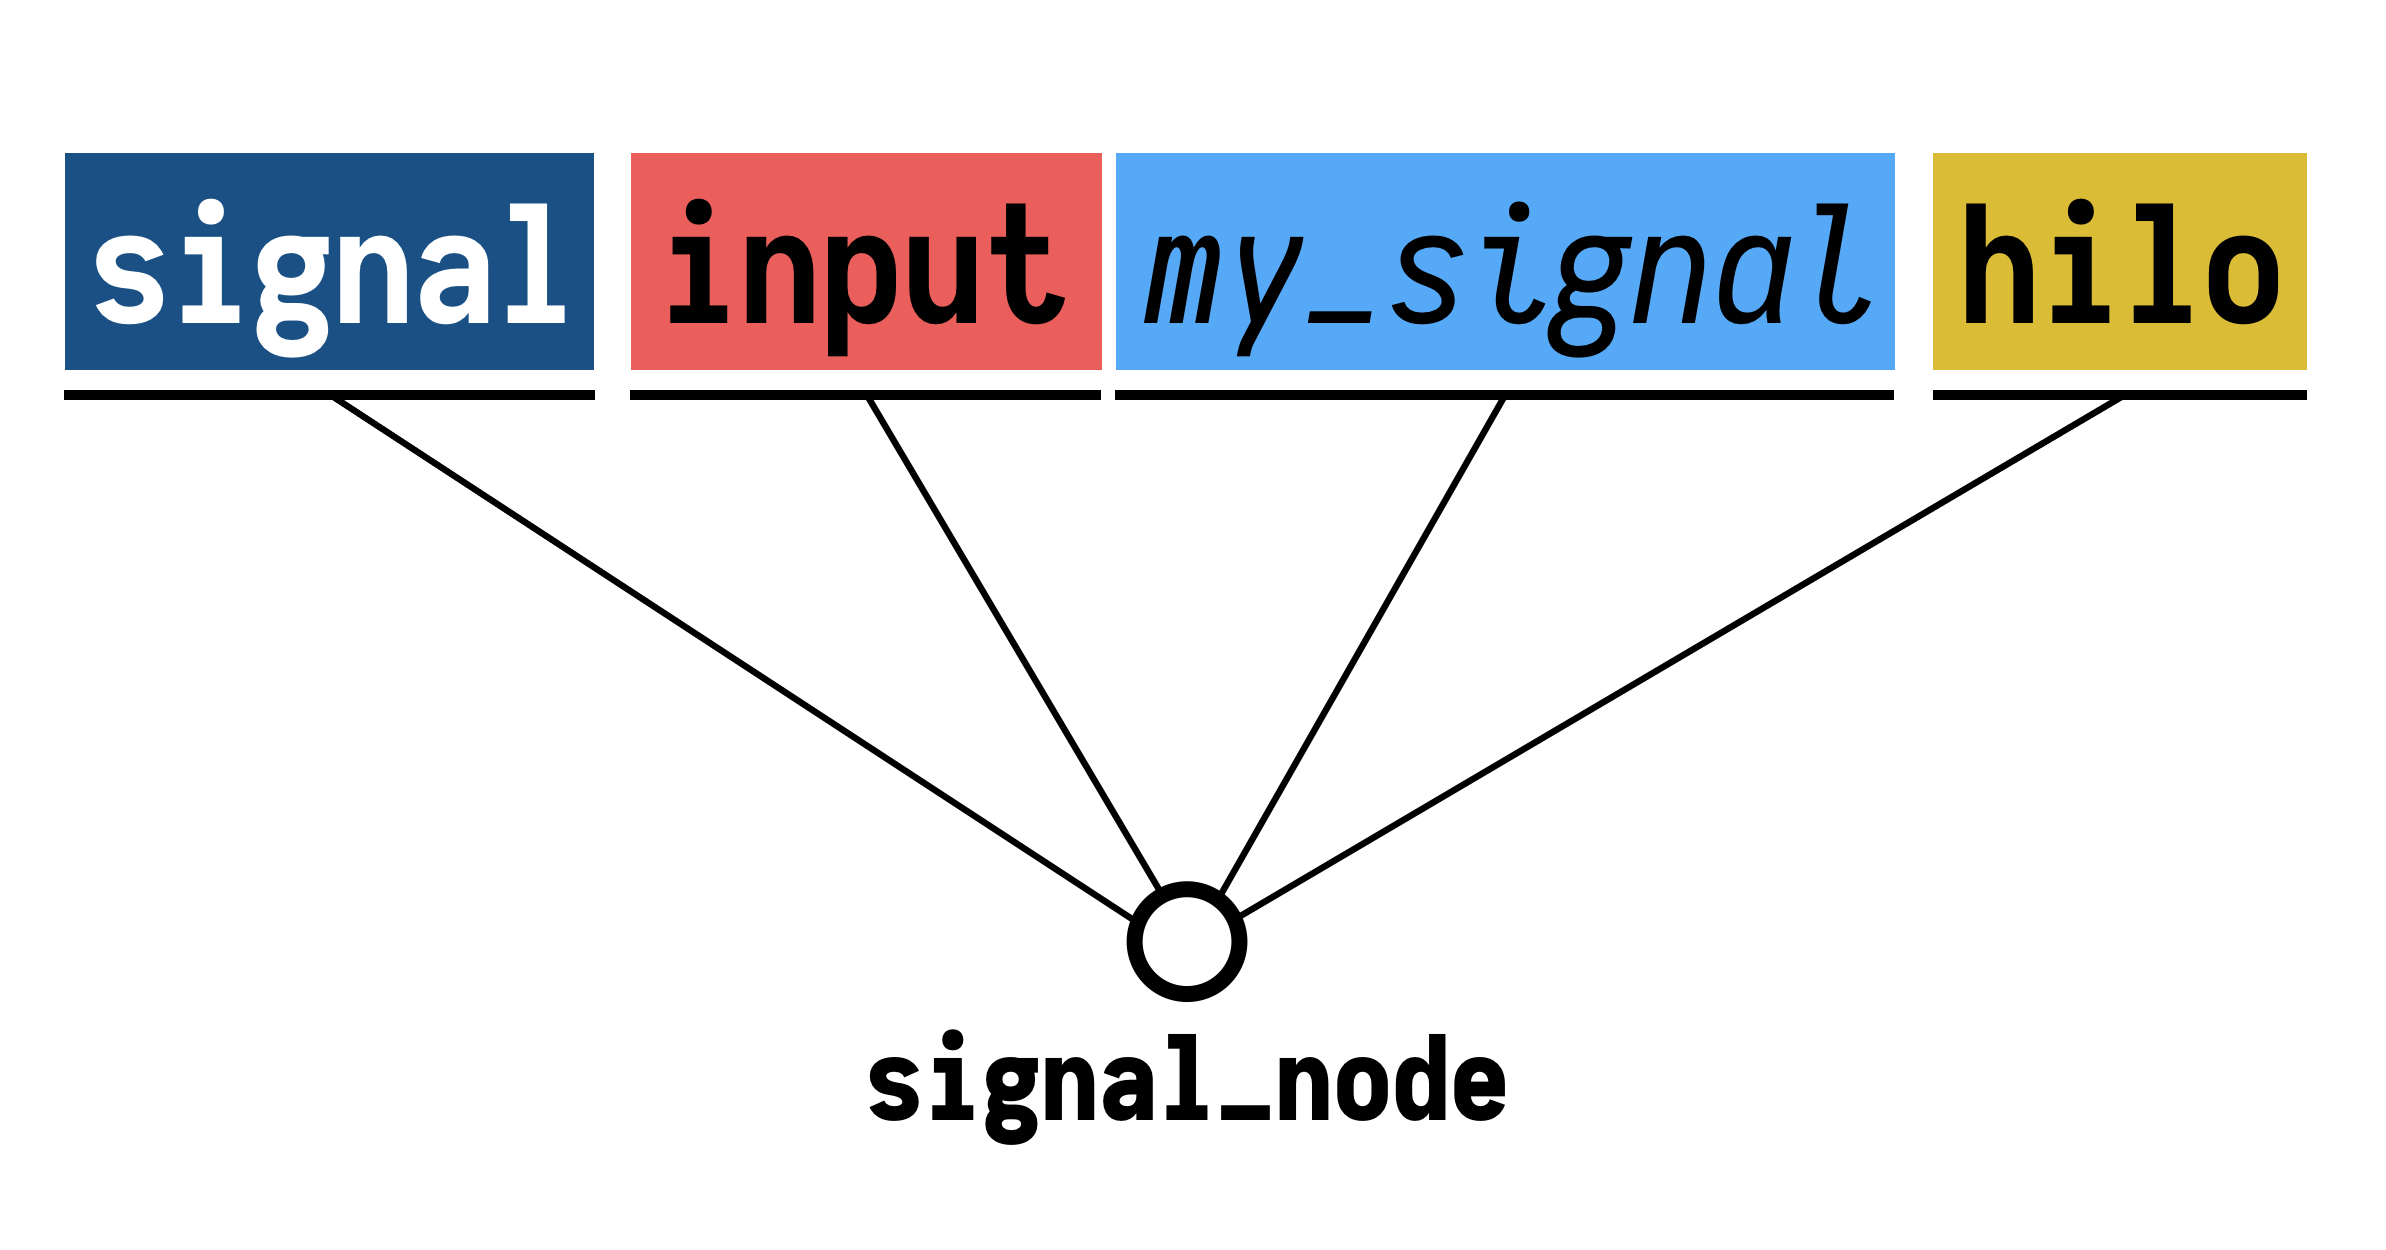
\includegraphics[height=5cm]{res/parser.png}
    \caption{Beispiel: Hopperlang AST}\label{fig:ast}
\end{figure}

\section{Aufgabenstellung}

Ziel des Moduls war eine Sprache zu entwerfen, die den Entwurf von VHDL Automaten vereinfacht.
Dabei sollen die Automatenschnittstellen und die Zustandsübergänge festgelegt werden können.

\section{Sprachaufbau}

Unsere Inspiration für Hopperlang waren Ruby und Go.

Von Ruby haben wir die lesbare Syntax abgeleitet und von Go kommt die Reihenfolge der Komponenten der Variablen-Deklaration, sowie die Deklarationsblöcke.

\subsection{Datentypen}

\begin{listing}[H]
\begin{itemize}
    \item \mintinline{hlang}{hilo} - ein Bit, high oder low (1 / 0), entspricht VHDL \mintinline{vhdl}{std_logic}
    \item \mintinline{hlang}{bus8} - ein Bitarray mit Breite 8, entspricht VHDL \mintinline{vhdl}{std_logic_vector}
    \item \mintinline{hlang}{int8} - eine vorzeichenlose Ganzzahl mit Größe 256, entspricht VHDL \mintinline{vhdl}{integer}
\end{itemize}
Die Datentypen \mintinline{hlang}{bus_} und \mintinline{hlang}{int_} sind in ihrer Größe einstellbar. Dabei sind Instanzen der gleichen Größe einander zuweisbar.
% \caption{Datentypen}
\label{lst:hl_types}
\end{listing}

\subsection{Deklarieren von Signalen}

\begin{listing}[H]
\begin{minted}{hlang}
signal input (
      clk   hilo
      reset hilo
      x     int8
)
signal output (
      y bus16
)
\end{minted}
% \caption{Deklarieren von Signalen}
\label{lst:hl_signals}
\end{listing}

\subsection{Deklarieren des Automaten}

\begin{listing}[H]
\begin{minted}{hlang}
automat my_automat do
    # signal declarations here
end
\end{minted}
% \caption{Deklarieren des Automaten}
\label{lst:hl_autom}
\end{listing}

\subsection{Übergangsbedingungen}

\begin{listing}[H]
\begin{minted}{hlang}
when (x=1) do
    when (y=4)     goto s0
    when not (y=0) goto s1
    x=0
end
\end{minted}
% \caption{Übergangsbedingungen}
\label{lst:hl_when}
\end{listing}

\subsection{Deklarieren von Zuständen}

\begin{listing}[H]
\begin{minted}{hlang}
state s0 do
  # conditions here
end

state s1 do
  # conditions here
end
\end{minted}
% \caption{Deklarieren von Zuständen}
\label{lst:hl_states}
\end{listing}

\newpage
\section{Aufbau des Hopperlang Compilers}

\end{document}
